\documentclass[]{article}
\usepackage{lmodern}
\usepackage{amssymb,amsmath}
\usepackage{ifxetex,ifluatex}
\usepackage{fixltx2e} % provides \textsubscript
\ifnum 0\ifxetex 1\fi\ifluatex 1\fi=0 % if pdftex
  \usepackage[T1]{fontenc}
  \usepackage[utf8]{inputenc}
\else % if luatex or xelatex
  \ifxetex
    \usepackage{mathspec}
  \else
    \usepackage{fontspec}
  \fi
  \defaultfontfeatures{Ligatures=TeX,Scale=MatchLowercase}
\fi
% use upquote if available, for straight quotes in verbatim environments
\IfFileExists{upquote.sty}{\usepackage{upquote}}{}
% use microtype if available
\IfFileExists{microtype.sty}{%
\usepackage[]{microtype}
\UseMicrotypeSet[protrusion]{basicmath} % disable protrusion for tt fonts
}{}
\PassOptionsToPackage{hyphens}{url} % url is loaded by hyperref
\usepackage[unicode=true]{hyperref}
\hypersetup{
            pdfborder={0 0 0},
            breaklinks=true}
\urlstyle{same}  % don't use monospace font for urls
\usepackage[margin=1in]{geometry}
\usepackage{graphicx,grffile}
\makeatletter
\def\maxwidth{\ifdim\Gin@nat@width>\linewidth\linewidth\else\Gin@nat@width\fi}
\def\maxheight{\ifdim\Gin@nat@height>\textheight\textheight\else\Gin@nat@height\fi}
\makeatother
% Scale images if necessary, so that they will not overflow the page
% margins by default, and it is still possible to overwrite the defaults
% using explicit options in \includegraphics[width, height, ...]{}
\setkeys{Gin}{width=\maxwidth,height=\maxheight,keepaspectratio}
\IfFileExists{parskip.sty}{%
\usepackage{parskip}
}{% else
\setlength{\parindent}{0pt}
\setlength{\parskip}{6pt plus 2pt minus 1pt}
}
\setlength{\emergencystretch}{3em}  % prevent overfull lines
\providecommand{\tightlist}{%
  \setlength{\itemsep}{0pt}\setlength{\parskip}{0pt}}
\setcounter{secnumdepth}{0}
% Redefines (sub)paragraphs to behave more like sections
\ifx\paragraph\undefined\else
\let\oldparagraph\paragraph
\renewcommand{\paragraph}[1]{\oldparagraph{#1}\mbox{}}
\fi
\ifx\subparagraph\undefined\else
\let\oldsubparagraph\subparagraph
\renewcommand{\subparagraph}[1]{\oldsubparagraph{#1}\mbox{}}
\fi

% set default figure placement to htbp
\makeatletter
\def\fps@figure{htbp}
\makeatother

\usepackage{ctex}
\usepackage{xcolor}
\usepackage{fancyhdr}
\pagestyle{plain}
\usepackage{sectsty}
\definecolor{glaucous}{rgb}{0.38, 0.51, 0.71}
\definecolor{lavenderblush}{rgb}{1.0, 0.94, 0.96}
\definecolor{grey}{RGB}{96, 96, 96}
\usepackage{enumitem}% http://ctan.org/pkg/enumitem
\usepackage[empty]{fullpage}% http://ctan.org/pkg/fullpage
\usepackage{color}% http://ctan.org/pkg/color
\usepackage{hyperref}% http://ctan.org/pkg/hyperref
\usepackage{geometry}
\geometry{papersize={15.5cm,50cm},left=0.5cm,right=0.5cm,top=0.3cm,bottom=0.3cm}
\usepackage{blindtext}
\usepackage[center]{caption}
\usepackage[font=Large]{caption}
\usepackage{subfigure}
\usepackage{float}
\usepackage{graphicx}
\usepackage{booktabs}
\usepackage[justification=centering]{caption}
\usepackage{threeparttable}
\usepackage{longtable}
\usepackage{array}
\usepackage{multirow}
\usepackage{wrapfig}
\usepackage{float}
\usepackage{colortbl}
\usepackage{pdflscape}
\usepackage{tabu}
\usepackage{threeparttable}
\usepackage{threeparttablex}
\usepackage[normalem]{ulem}
\usepackage{makecell}
\usepackage{xcolor}
\linespread{1.85}
\setlength{\parskip}{1em}
\setlength{\footskip}{20pt}
\usepackage{booktabs}
\usepackage{longtable}
\usepackage{array}
\usepackage{multirow}
\usepackage{wrapfig}
\usepackage{float}
\usepackage{colortbl}
\usepackage{pdflscape}
\usepackage{tabu}
\usepackage{threeparttable}
\usepackage{threeparttablex}
\usepackage[normalem]{ulem}
\usepackage{makecell}
\usepackage{xcolor}

\author{}
\date{\vspace{-2.5em}}

\begin{document}

\captionsetup[figure]{name={图},labelsep=space}
\captionsetup[table]{name={表},labelsep=space} \fontsize{22}{22}
\selectfont
\vspace{-10truemm}

\newcommand{\resheading}[1]{%
  \noindent\fcolorbox{lavenderblush}{lavenderblush}{\makebox[\dimexpr\textwidth-2\fboxsep-2\fboxrule][c]{\textbf{~#1}}}%
}

\begin{center}

\includegraphics[height=2cm]{./input/logo2.png} 
\end{center}

\begin{center}
\fontsize{45}{45}
\textcolor{glaucous}{\textbf{新冠早报}}
\end{center}

\begin{center}
\fontsize{22}{22}
{\textcolor{glaucous}{\textbf{第77期 \space 7月7日}}}
\end{center}

\vspace{2mm}

\begin{center}

\includegraphics[height=2cm]{./input/title1.png} 
\end{center}

\vspace{-5mm}

\begin{huge}{\textcolor{glaucous}{\textbf{国际}}}\end{huge}

\vspace{-3mm}

\begin{center}
\textcolor{glaucous}{华盛顿邮报(The Washington Post)}\\239名科学家公开信:新冠可通过空气传播,建议WHO更新防护指南

\end{center}

据当地时间7月5日报道,来自32个国家的239名科学家近日联名给世界卫生组织发公开信指出,越来越多酒吧、餐厅、办公室等室内聚集感染为新冠病毒可以通过空气传播提供足够佐证,呼吁世卫组织承认新冠病毒空气传播的特性并更新防护指南。目前在截至6月29日世卫组织发布的预防新冠病毒传播的更新手册中,依然认为所谓的``空气传播''只有在产生气溶胶或小于5微米的病毒液滴的医疗操作环境下才有可能。

\begin{center}
\textcolor{glaucous}{美国移民与海关执法局(ICE)}\\美国:如果大学转为网上授课 国际学生或需离开美国
\end{center}

当地时间7月6日,美国移民与海关执法局(ICE)发布新规定,如果国际学生就读的美国高校在今年9月选择继续网上授课,美国国务院将不会给这些学生发放入境签证,且海关与边境保卫局不会允许这些学生入境,目前人在美国的国际学生也需要立即离境,或转至当面授课的高校就读。

\begin{center}
\textcolor{glaucous}{华盛顿邮报(The Washington Post)}\\美国前药监局专员:算上未诊断的病例,美国每天可能有70万例感染
\end{center}

当地时间7月6日,美国前药监局专员斯科特·戈特利布在采访中表示,美国目前可能仅诊断出十二分之一的新冠病毒病例,这意味着每天新增真实感染的数量可能很快达到70万例。

\begin{center}
\textcolor{glaucous}{英国广播公司(BBC)}\\英国解封:周末酒吧重开,人潮汹涌
\end{center}

当地时间7月4日,英格兰酒吧餐厅恢复营业,大批人潮晚间聚集在伦敦苏豪区饮酒作乐,现场挤得水泄不通,几乎没人保持安全社交距离。当地警察表示,苏豪区人潮到周日凌晨才逐渐散去,好在并没有发生``严重事故''。

\begin{center}
\textcolor{glaucous}{法国国际广播电台(rfi)}\\卢浮宫重开,游客保持距离欣赏蒙娜丽莎
\end{center}

当地时间7月6日,巴黎卢浮宫重新对外开放。马蒂内馆长表示,关闭三个半月后重新开放的博物馆和历史古迹采取``一切措施''保障工作人员和参观者的健康。如今长期闭馆已致卢浮宫亏损4千万欧元,而开馆后卢浮宫的参观人数预计将减少80\%。

\begin{center}
\textcolor{glaucous}{新浪新闻}\\印度新冠确诊病例已经超过俄罗斯,成为全球第三
\end{center}

当地时间7月5日,印度超过俄罗斯成为全球新冠肺炎确诊病例第三多的国家。印度当日通报近2.5万例新增病例,累计确诊病例将近70万。

\vspace{5mm}

\begin{huge}{\textcolor{glaucous}{\textbf {国内}}}\end{huge}

\vspace{-3mm}

\begin{center}
\textcolor{glaucous}{新浪新闻}\\7.4万名北京新发地相关人员隔离期满
\end{center}

北京时间7月5日,曾去过新发地市场牛羊肉综合交易大楼的人员及其同住人员共7.4万人,延长居家观察已满7天,完成了``14+7''天的隔离观察,已有序组织第三次核酸检测,检测结果为阴性且体温等症状排查无异常者,即可解除居家隔离观察。此外,新发地牛羊肉综合交易大楼工作人员仍要采取``14+14''天的隔离观察措施。

\vspace{10mm}

\begin{center}

\includegraphics[height=2cm]{./input/title2.png} 
\end{center}

\begin{Large}
\vspace{-7mm}
{数据源:约翰霍普金斯大学,The COVID Tracking  Project}
\end{Large}

\vspace{-7mm}

\begin{Large}
{数据截止至:北京时间7月7日 上午8:30}
\end{Large}

\begin{huge}{\textcolor{glaucous}{\textbf {一、世界疫情}}}\end{huge}

\vspace{-5mm}

\(\bullet\)全球累计确诊病例达11,589,066例,累计死亡537,413例。共有34个国家累计确诊病例数超过5万例,其中12个为亚洲国家,11个为欧洲国家,9个为美洲国家,另有2个非洲国家。

\(\quad\)\(\diamond\)北美洲地区疫情蔓延迅速,截止至今日,累计确诊病例数超过340万例,排名第一。

\(\quad\)\(\diamond\)南美洲,亚洲以及欧洲确诊病例数持续增长,直至今日,确诊病例数均超过250万例。

\begin{figure}[H]

\caption{世界疫情分布趋势图\\ \vspace{-3mm}(来源:WHO)} %最终文档中希望显示的图片标题
\centering
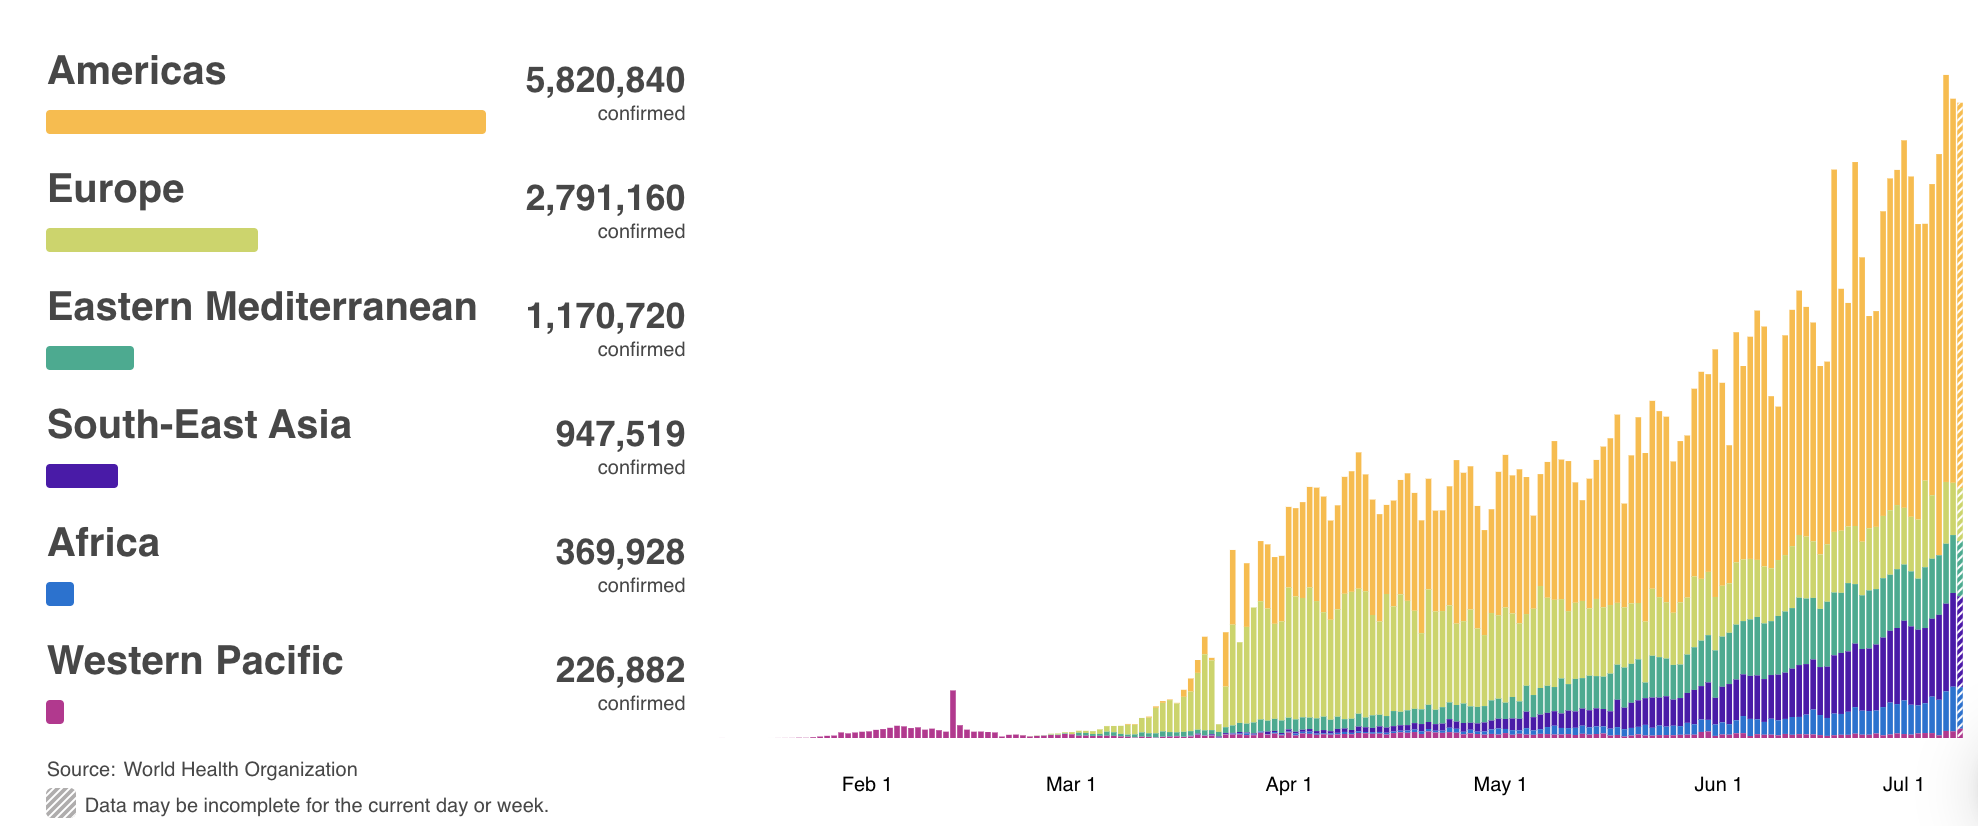
\includegraphics[]{./input/covid1.png} %插入图片,[]中设置图片大小,{}中是图片文件名
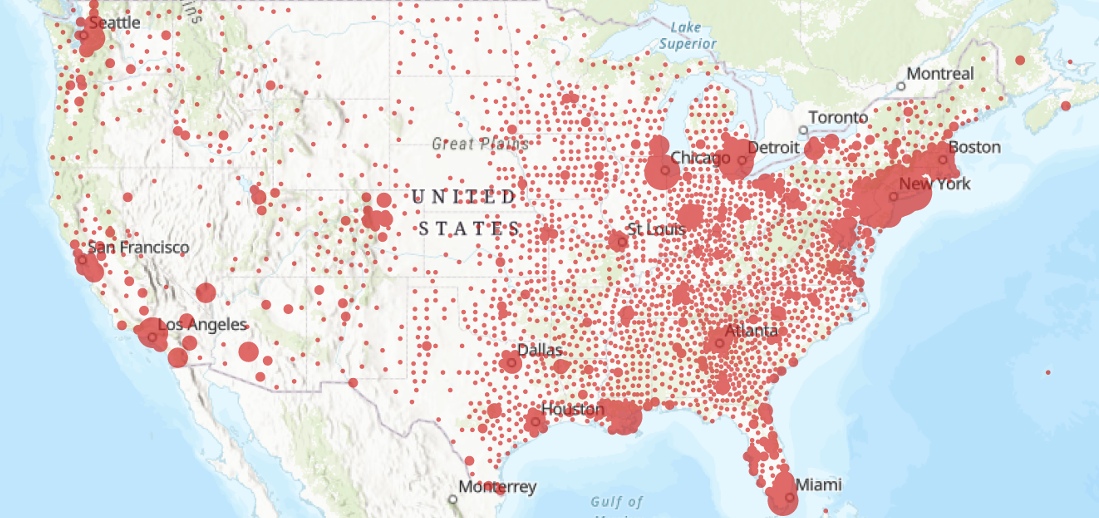
\includegraphics[]{./input/covid4.png}
\label{} %用于文内引用的标签
\end{figure}

\begin{table}[H]
    \centering \begin{table}[H]
\centering\begingroup\fontsize{14}{16}\selectfont

\begin{tabular}{rlrrrr}
\toprule
\multicolumn{0}{c}{\textbf{ }} & \multicolumn{3}{c}{\textbf{表1 累计确诊前十位国家}} \\
  & 国家(地区) & 累计确诊 & 粗发病率* & 累计死亡 & 病死率\%\\
\midrule
\rowcolor{gray!6}  1 & 美国 US & 2,934,499 & 887 & 130,271 & 4.4\\
2 & 巴西 Brazil & 1,623,284 & 764 & 65,487 & 4.0\\
\rowcolor{gray!6}  3 & 印度 India & 697,413 & 51 & 19,693 & 2.8\\
4 & 俄罗斯 Russia & 686,777 & 471 & 10,271 & 1.5\\
\rowcolor{gray!6}  5 & 秘鲁 Peru & 305,703 & 927 & 10,772 & 3.5\\
6 & 智利 Chile & 298,557 & 1,562 & 6,384 & 2.1\\
\rowcolor{gray!6}  7 & 英国 UK & 287,290 & 423 & 44,321 & 15.4\\
8 & 墨西哥 Mexico & 261,750 & 203 & 31,119 & 11.9\\
\rowcolor{gray!6}  9 & 西班牙 Spain & 251,789 & 539 & 28,752 & 11.4\\
10 & 伊朗 Iran & 243,051 & 289 & 11,731 & 4.8\\
\bottomrule
\end{tabular}
\endgroup{}
\end{table} \begin{tablenotes}
        \fontsize{15}{15}
        \selectfont
        \item 注:*粗发病率定义:在一定时间内,特定范围人群中某病新发生的病例出现的频率。计算方式:(累计确诊病例/人口)×10万;国家人口不足 10 万人未列出 %此处加入注释信息
      \end{tablenotes}
\end{table}

\begin{table}[H]
   \centering \begin{table}[H]
\centering\begingroup\fontsize{18}{20}\selectfont

\begin{tabular}{rlrr}
\toprule
\multicolumn{0}{c}{\textbf{ }} & \multicolumn{2}{c}{\textbf{表2 日新增病例前十位国家}} \\
  & 国家 & 新增确诊 & 新增死亡\\
\midrule
\rowcolor{gray!6}  1 & 美国 US & 45,864 & 324\\
2 & 印度 India & 24,248 & 0\\
\rowcolor{gray!6}  3 & 巴西 Brazil & 20,229 & 620\\
4 & 南非 South Africa & 8,971 & 111\\
\rowcolor{gray!6}  5 & 巴基斯坦 Pakistan & 6,535 & 0\\
6 & 俄罗斯 Russia & 6,494 & 126\\
\rowcolor{gray!6}  7 & 墨西哥 Mexico & 4,902 & 480\\
8 & 沙特 Saudi Arabia & 4,207 & 52\\
\rowcolor{gray!6}  9 & 哥伦比亚 Colombia & 3,727 & 127\\
10 & 孟加拉国 Bangladesh & 3,201 & 44\\
\bottomrule
\end{tabular}
\endgroup{}
\end{table} \end{table}

\(\bullet\)全球昨日新增确诊接近14万例(139,672例),新增死亡3,152例(表2)。

\(\quad\)\(\diamond\)北美洲新增确诊接近5.5万例,新增死亡890例。其中虽然美国今日新增病例数较前几日有所下降,但依旧占北美洲日新增确诊数的近85\%。

\(\quad\)\(\diamond\)南美洲新增确诊超过2.5万例,新增死亡超过1,100例,超过80\%的日新增确诊和超过一半的新增死亡病例均来自巴西。截止今日,巴西连续10日为全球日新增死亡病例最高的国家。值得注意的是,墨西哥近一周以来,日新病例数一直位于该地区第二,且自上周末起,其日新增死亡病例数始终位于世界第二。此外,该地区日新增病例数排名前列的国家哥伦比亚、秘鲁和智利近一周均在日新增确诊数3,000例上下波动。

\(\quad\)\(\diamond\)亚洲新增确诊约2.2万例,新增死亡591例。该地区疫情严重的国家沙特、孟加拉国和伊朗新增确诊均超过2,500例。

\(\quad\)\(\diamond\)非洲新增确诊接近1.4万例,新增死亡249例。南非疫情持续扩散,近一周单日新增确诊病例均在9,000例上下波动。

\vspace{-7mm}

\begin{figure}[H]
\centering

\vspace{2mm}
\caption{日新增确诊病例国家趋势图}
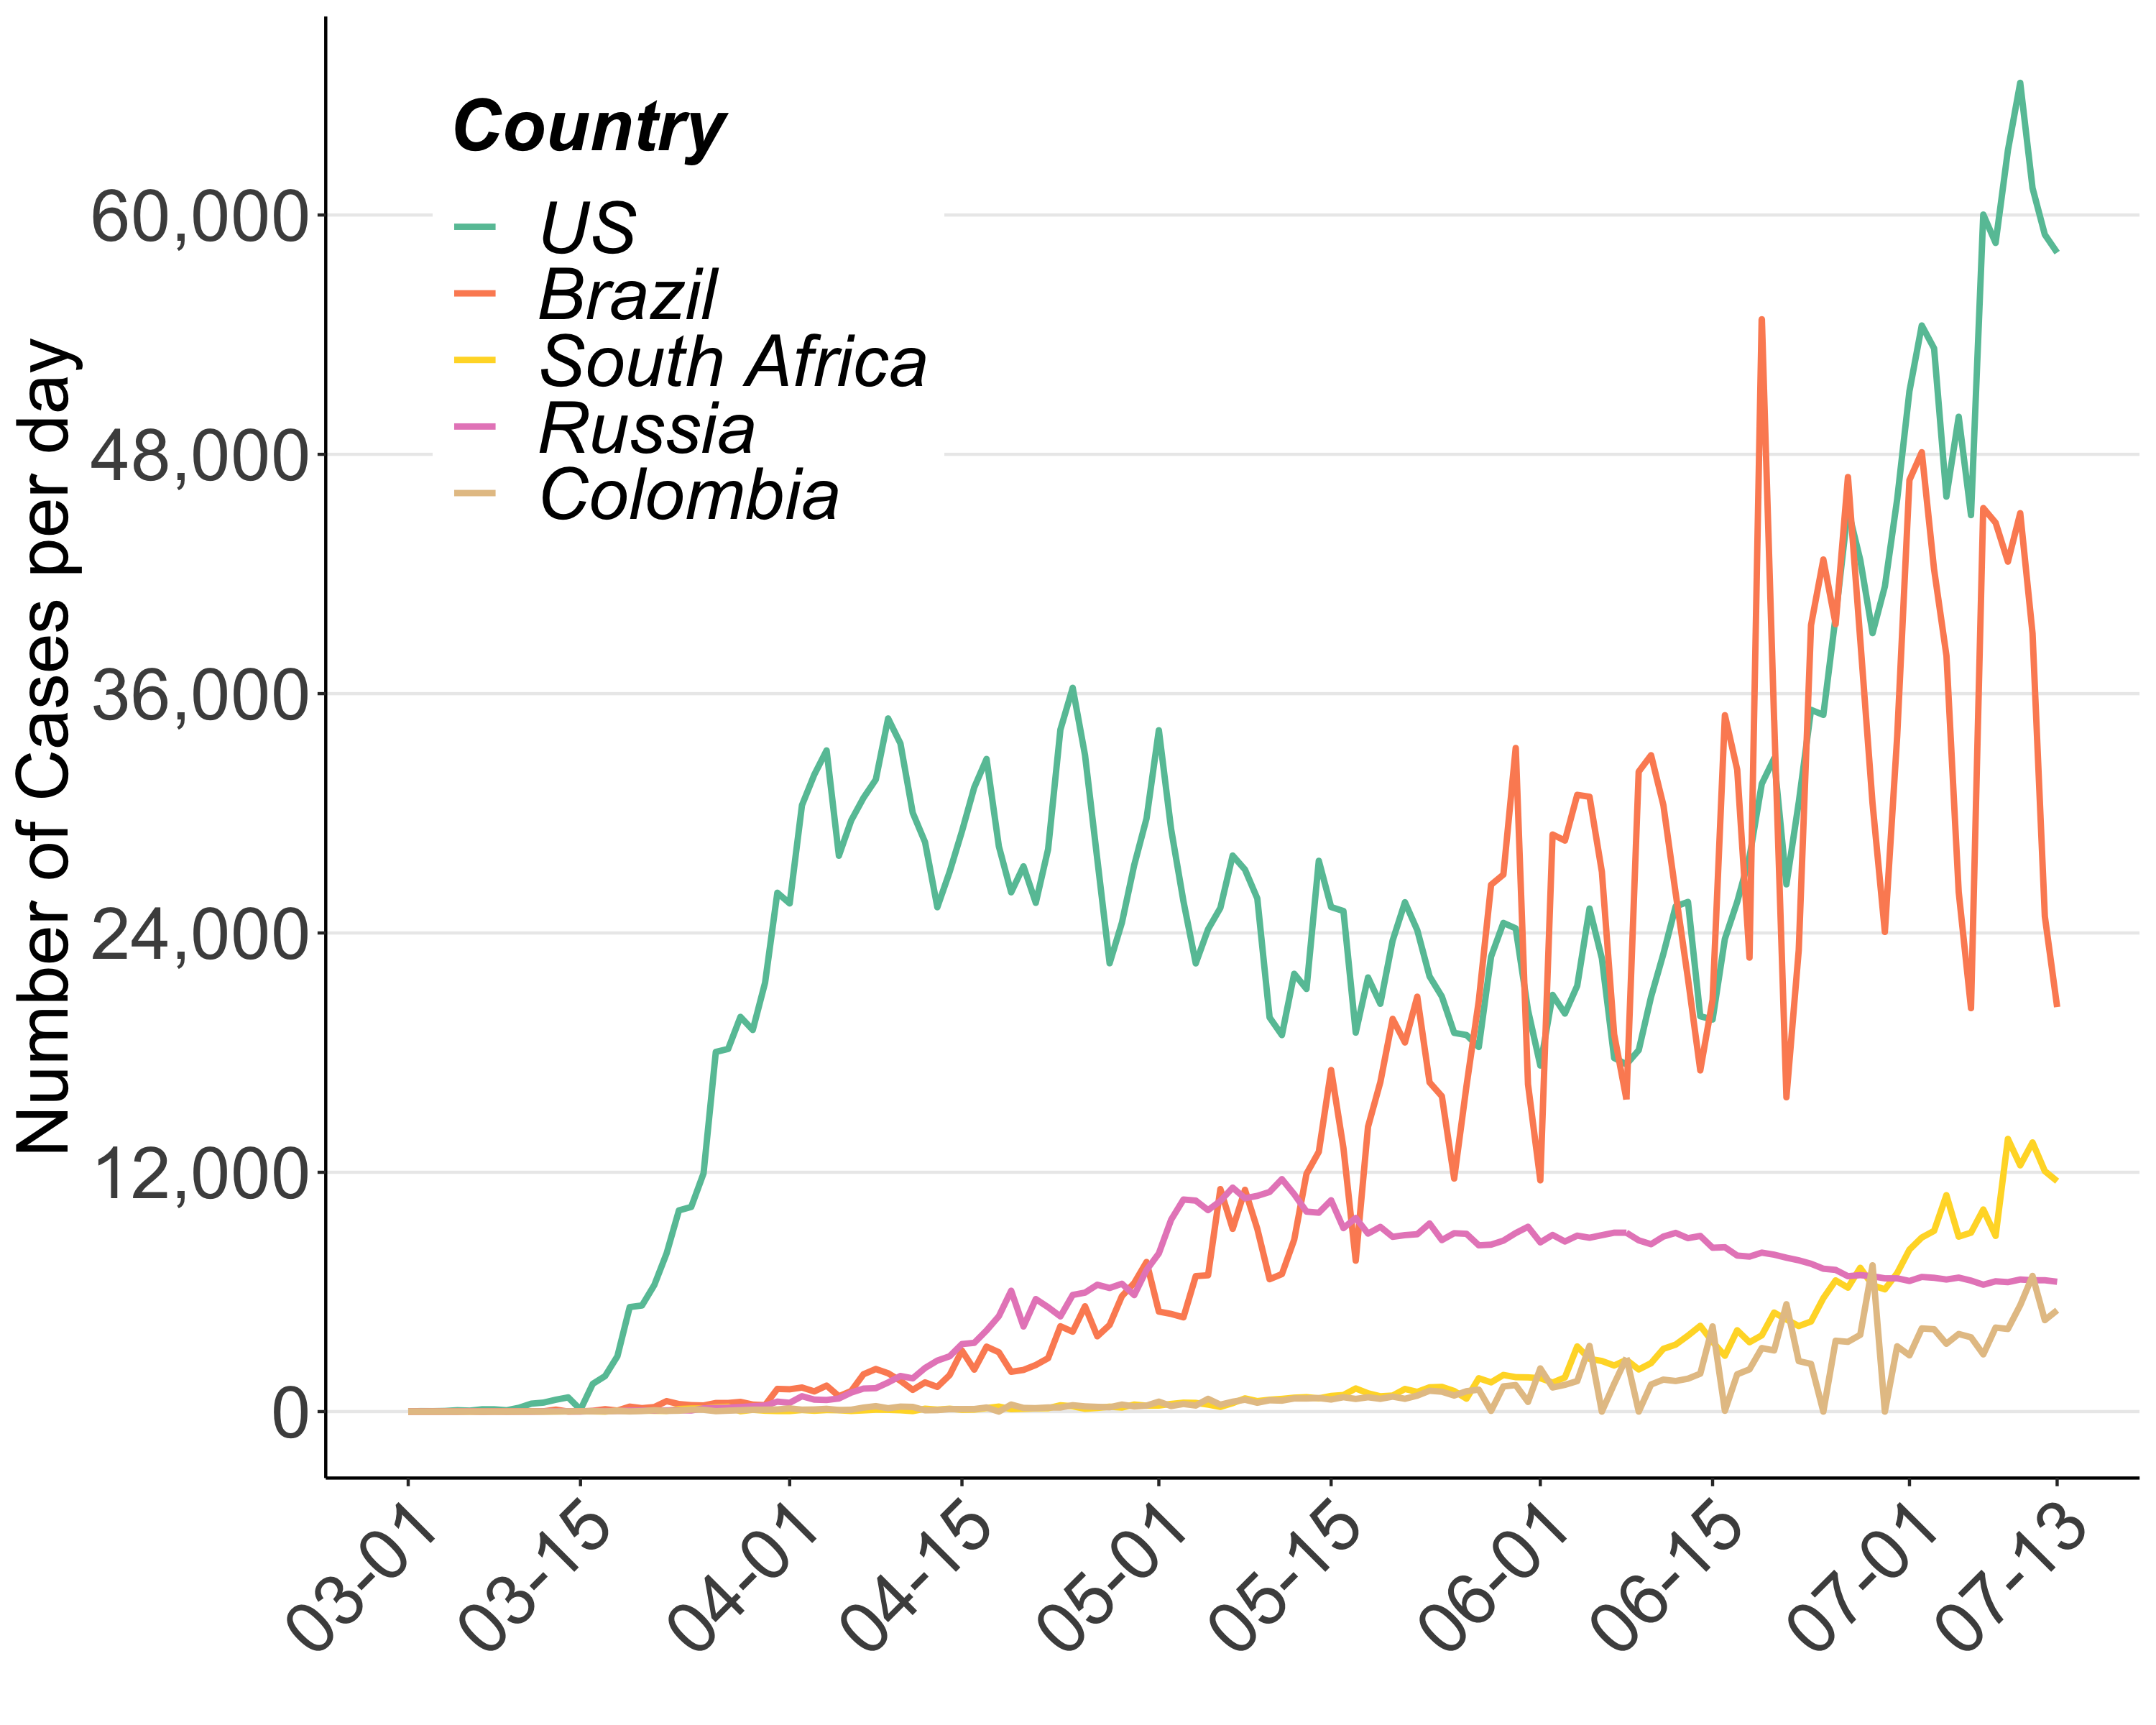
\includegraphics[]{./input/covid2.png}
\end{figure}

\begin{figure}[H]
\centering

\caption{日新增死亡病例国家趋势图}
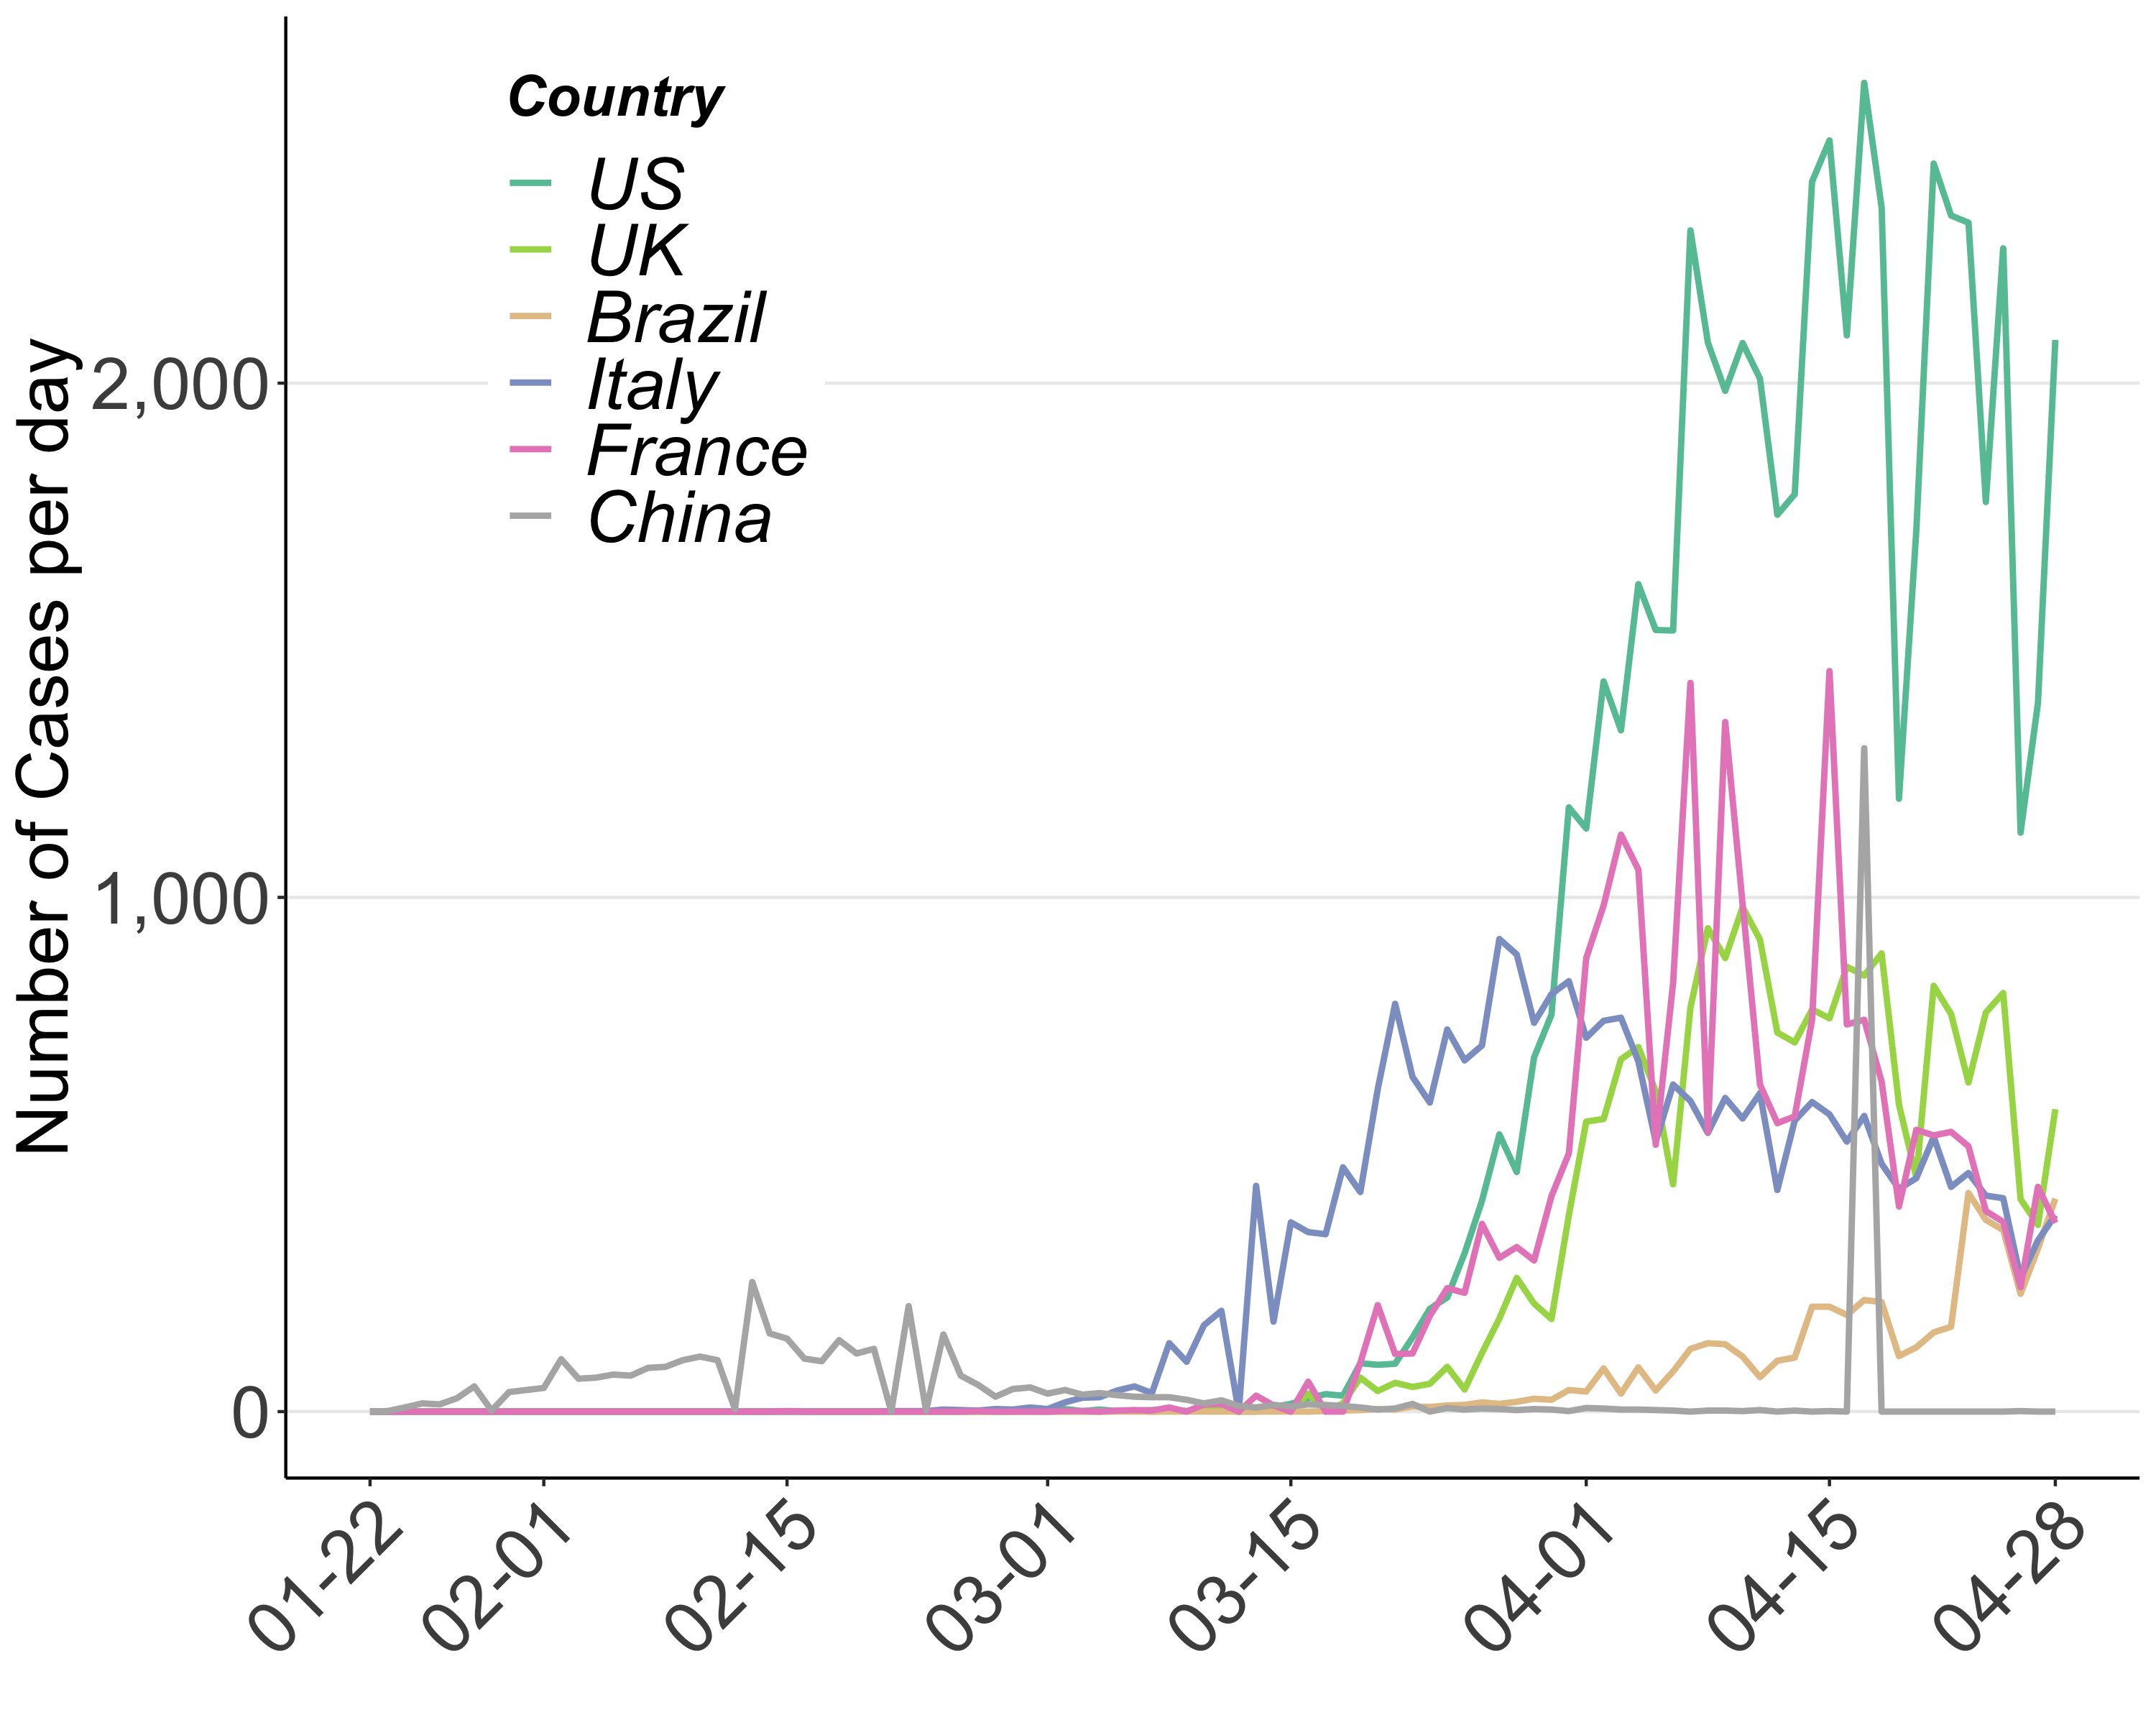
\includegraphics[]{./input/covid3.png}
\end{figure}

\vspace{-7mm}

\begin{huge}{\textcolor{glaucous}{\textbf {二、美国疫情}}}\end{huge}

\vspace{-5mm}

\(\bullet\)截至北京时间7月4日早8:30,
美国累计确诊病例数为2,934,499例,累计死亡130,271例。

\(\quad\)\(\diamond\)共有40个州及地区累计确诊病例超过1万例,17个州累计确诊病例超过5万例。

\vspace{2mm}

\begin{figure}[H]
\centering

\caption{美国日新增确诊前五位州趋势图}
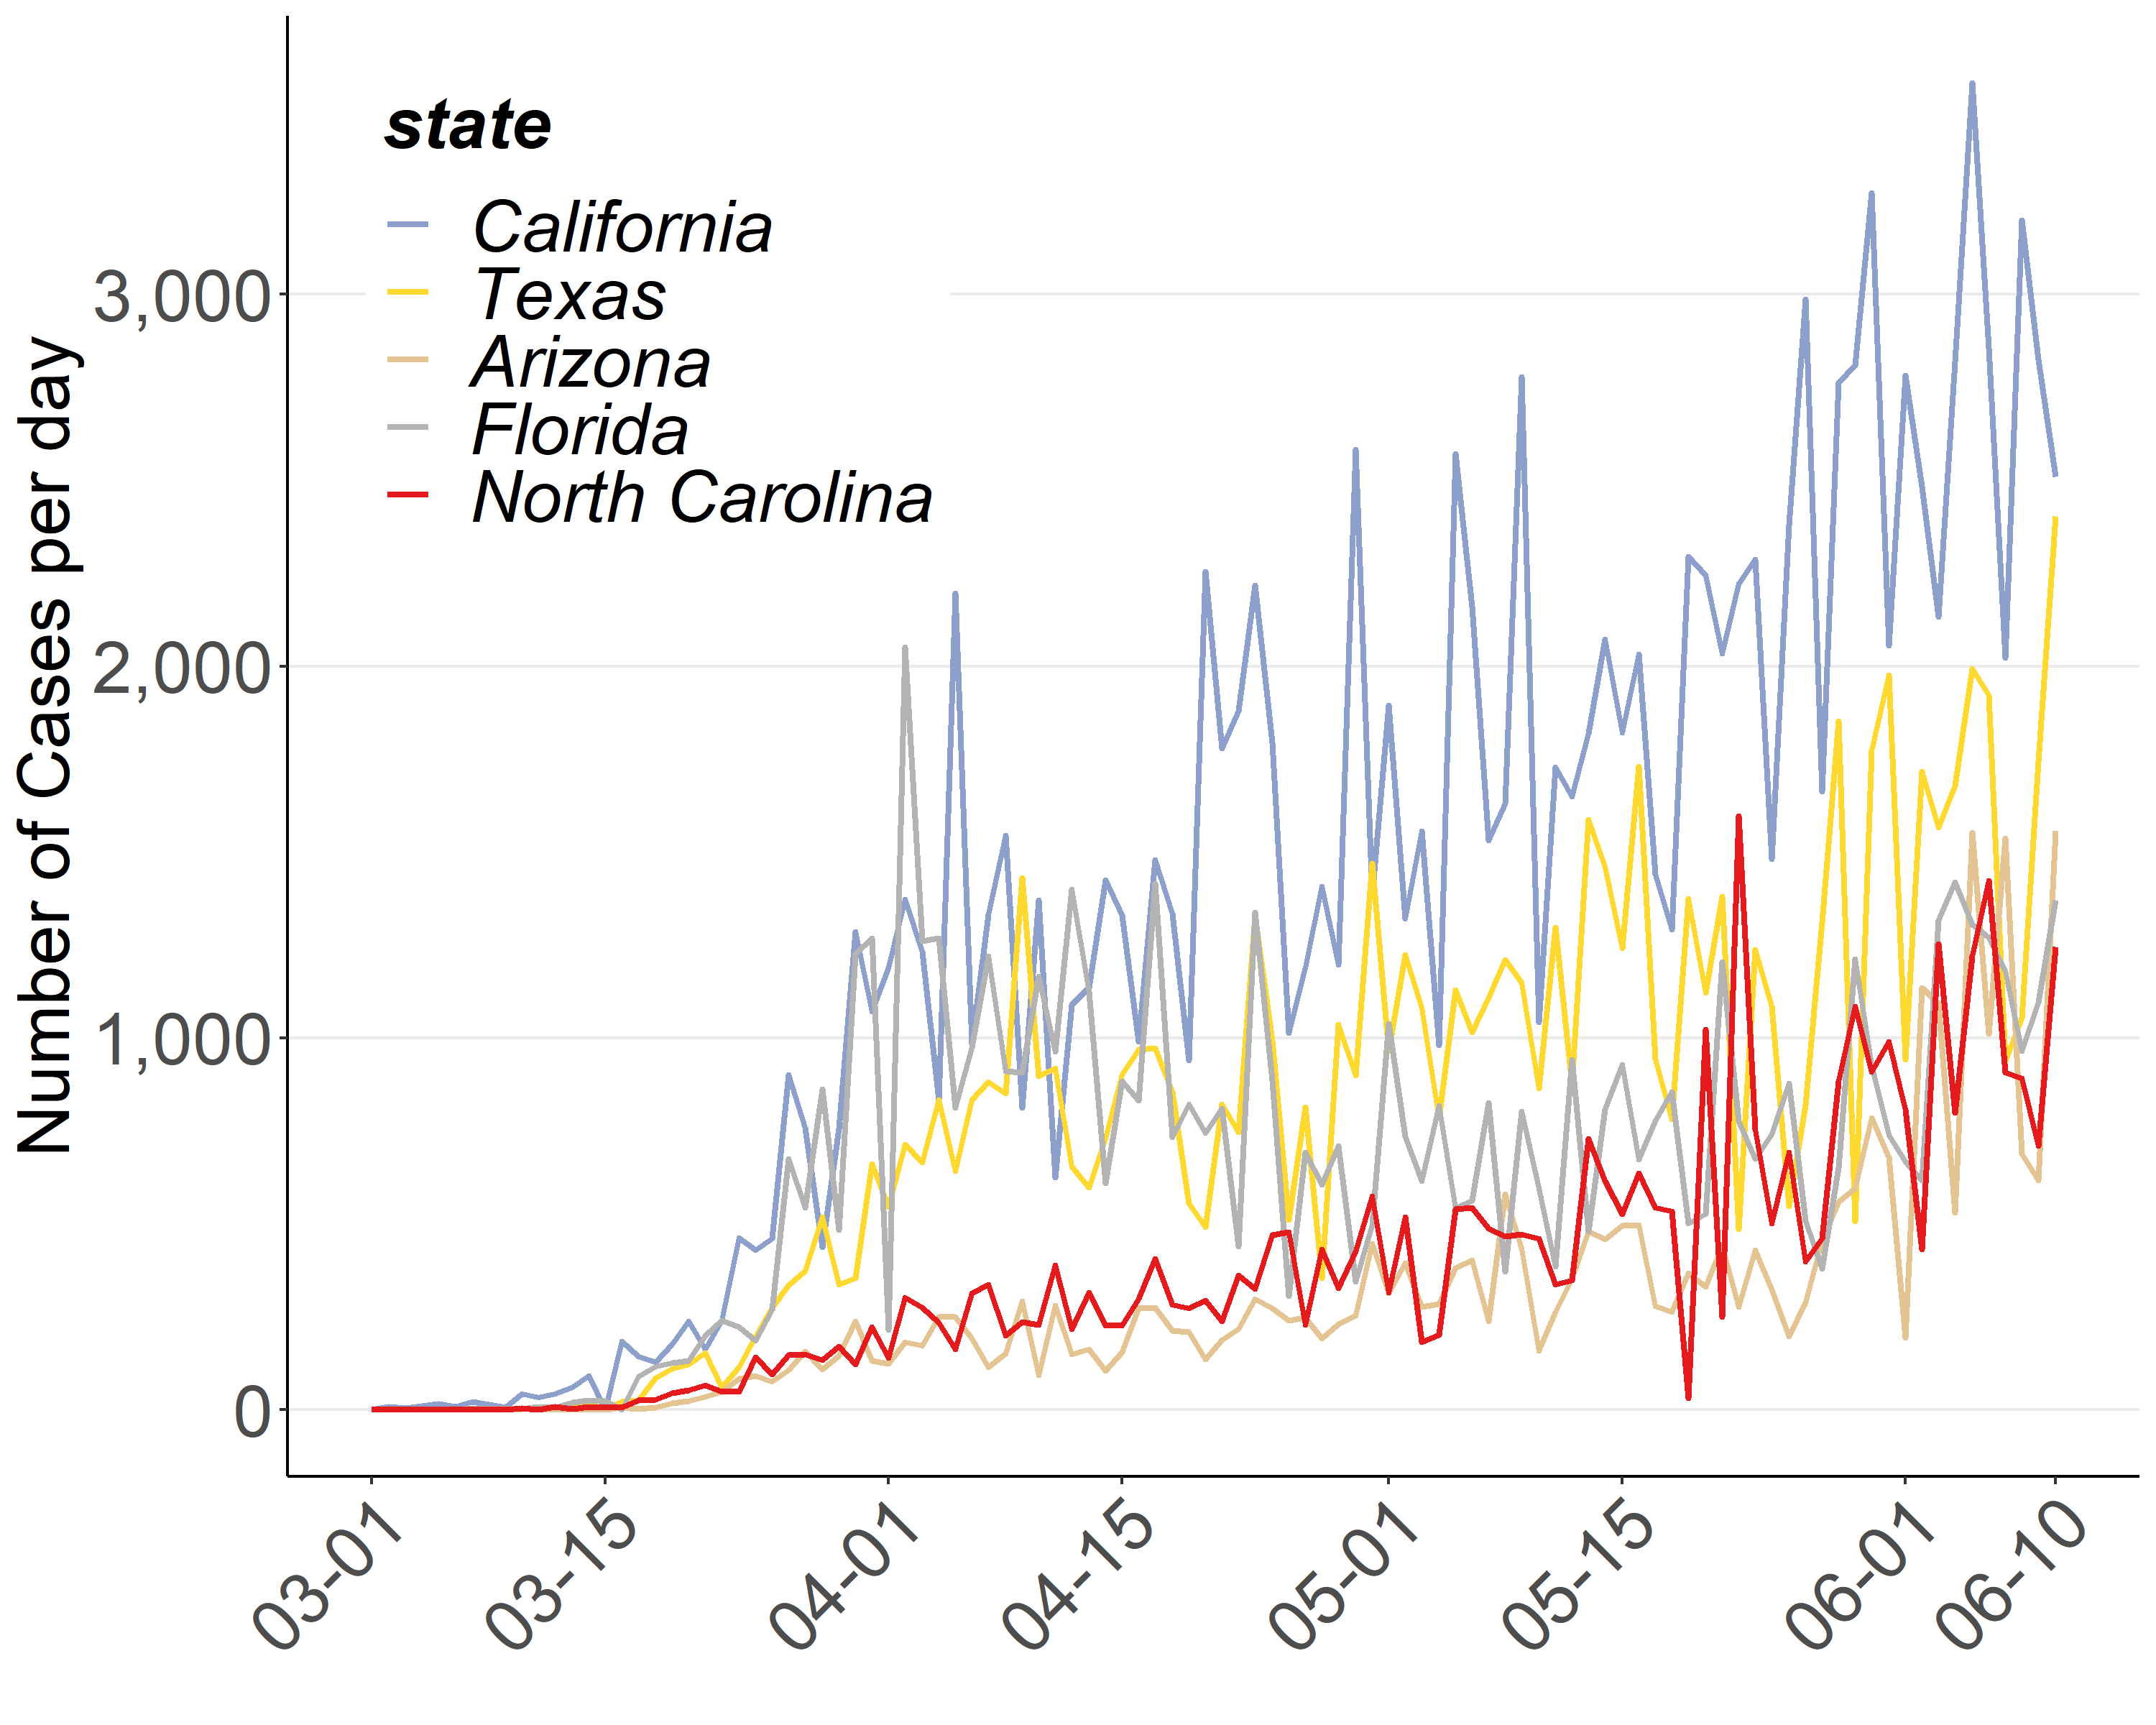
\includegraphics[]{./input/covid5.png}
\end{figure}

\begin{figure}[H]
\centering

\caption{美国日新增死亡前五位州趋势图}
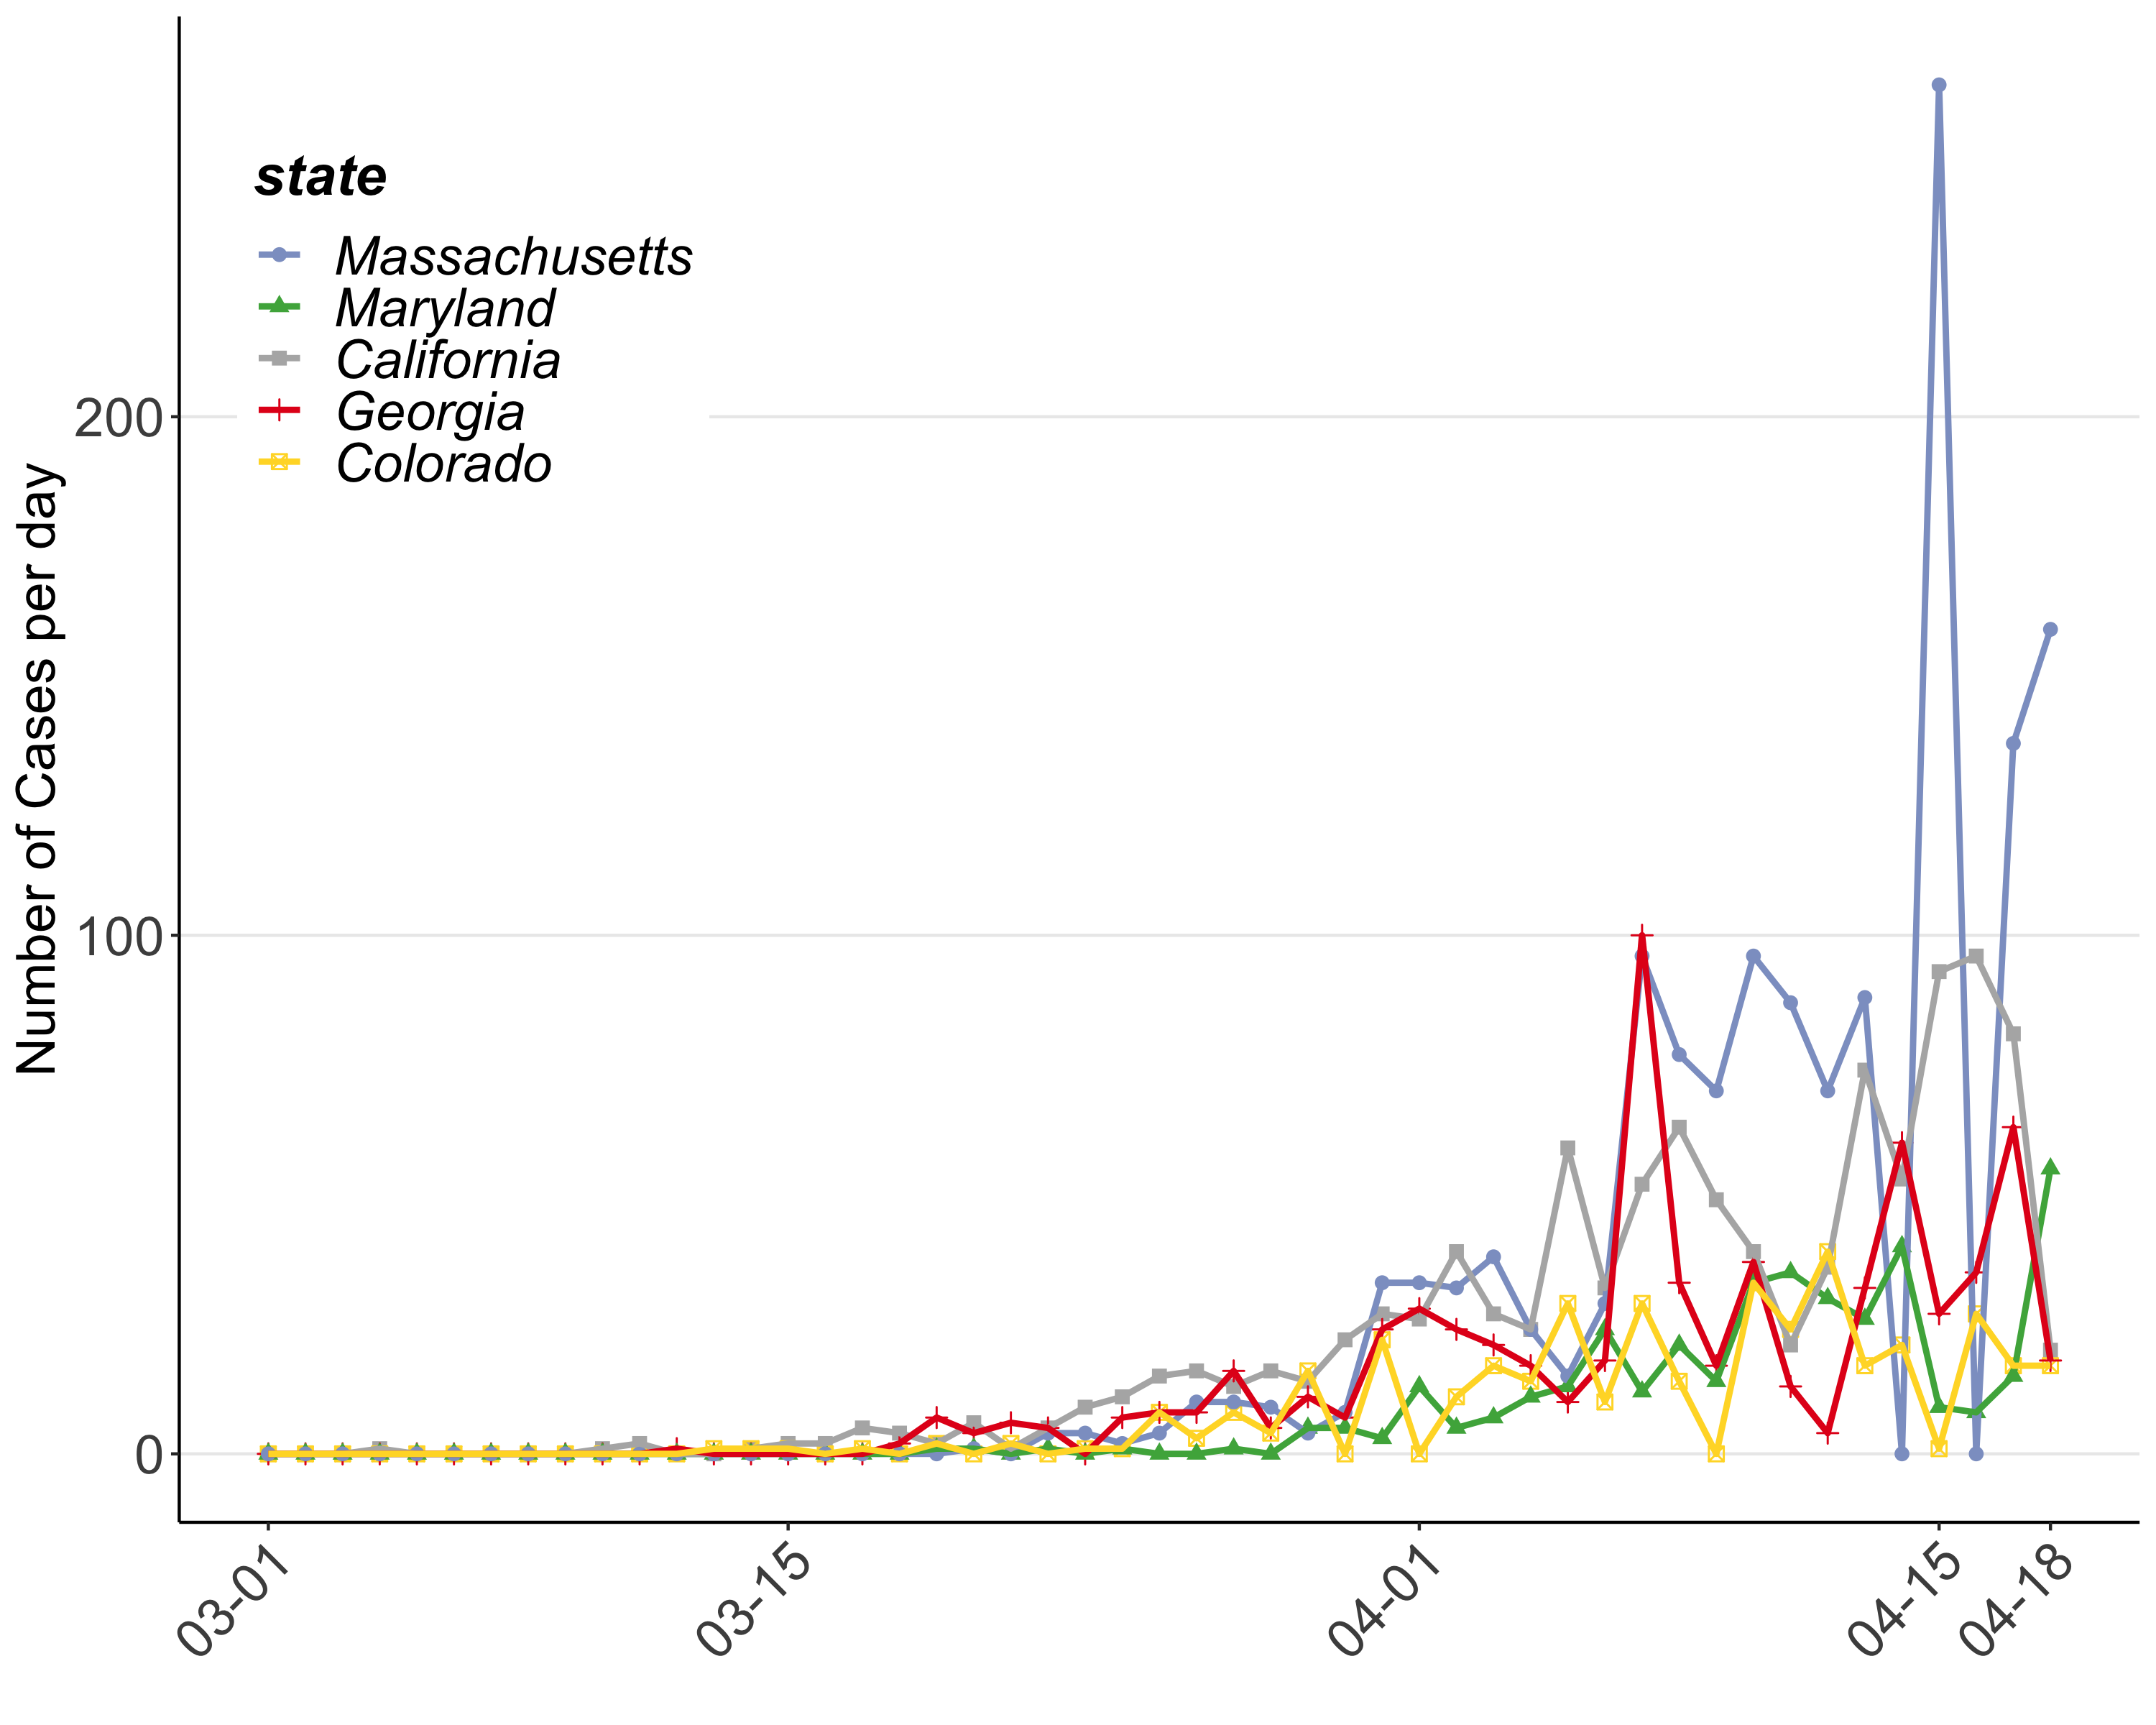
\includegraphics[]{./input/covid6.png}
\end{figure}

\begin{table}[H]
    \centering \begin{table}[H]
\centering\begingroup\fontsize{16}{18}\selectfont

\resizebox{\linewidth}{!}{
\begin{tabular}{rlrr}
\toprule
\multicolumn{0}{c}{\textbf{ }} & \multicolumn{3}{c}{\textbf{表3 美国新增确诊前十位州}} \\
  & 国家/州名 & 当日新增 & 累计确诊\\
\midrule
\rowcolor{gray!6}   & 美国 US & 45,864 & 2,934,499\\
1 & 得克萨斯州 TX & 10,704 & 205,636\\
\rowcolor{gray!6}  2 & 佛罗里达州 FL & 6,336 & 206,447\\
3 & 加利福尼亚州 CA & 6,332 & 271,013\\
\rowcolor{gray!6}  4 & 亚利桑那州 AZ & 3,352 & 101,455\\
5 & 北卡罗莱纳州 NC & 1,783 & 74,775\\
\rowcolor{gray!6}  6 & 乔治亚州 GA & 1,544 & 97,060\\
7 & 南卡罗来纳州 SC & 1,533 & 46,380\\
\rowcolor{gray!6}  8 & 路易斯安那州 LA & 1,101 & 66,327\\
9 & 华盛顿州 WA & 1,087 & 36,985\\
\rowcolor{gray!6}  10 & 阿拉巴马州 AL & 925 & 44,878\\
\bottomrule
\end{tabular}}
\endgroup{}
\end{table} \end{table}

\begin{table}[H]
    \centering \begin{table}[H]
\centering\begingroup\fontsize{18}{20}\selectfont

\resizebox{\linewidth}{!}{
\begin{tabular}{rlrrr}
\toprule
\multicolumn{0}{c}{\textbf{ }} & \multicolumn{4}{c}{\textbf{表4 美国新增死亡前十位州}} \\
  & 国家/州名 & 当日新增 & 累计死亡 & 病死率\%\\
\midrule
\rowcolor{gray!6}   & 美国 US & 324 & 130,271 & 4.4\\
1 & 加利福尼亚州 CA & 67 & 6,440 & 2.4\\
\rowcolor{gray!6}  2 & 佛罗里达州 FL & 47 & 3,778 & 1.8\\
3 & 得克萨斯州 TX & 47 & 2,675 & 1.3\\
\rowcolor{gray!6}  4 & 新泽西州 NJ & 18 & 15,229 & 8.8\\
5 & 乔治亚州 GA & 16 & 2,876 & 3.0\\
\rowcolor{gray!6}  6 & 俄亥俄州 OH & 16 & 2,927 & 5.1\\
7 & 马萨诸塞州 MA & 15 & 8,198 & 7.4\\
\rowcolor{gray!6}  8 & 纽约州 NY & 13 & 32,219 & 8.1\\
9 & 华盛顿州 WA & 10 & 1,369 & 3.7\\
\rowcolor{gray!6}  10 & 北卡罗莱纳州 NC & 9 & 1,432 & 1.9\\
\bottomrule
\end{tabular}}
\endgroup{}
\end{table} \begin{tablenotes}
        \fontsize{15}{15}
        \selectfont
        \item 
      \end{tablenotes}
\end{table}

\(\bullet\)美国今日新增确诊45,864例,新增死亡324例(表3和表4)。单日新增确诊排名前十位的州昨日新增均超过1,000例,共40个州累计确诊超过10,000例。

\(\quad\)\(\diamond\)加利福尼亚州疫情蔓延迅速,于上周末日新增病例数首次突破1万例。

\(\quad\)\(\diamond\)德克萨斯州疫情不容乐观,单日确诊数再创新高,今日日新增首次突破1万例。

\vspace{15mm}

\begin{center}

\includegraphics[height=2cm]{./input/title3.png} 
\end{center}

\vspace{-7mm}

\vspace{-5mm}

\section{\texorpdfstring{\textcolor{glaucous}{\Huge 治疗一次新冠的费用,能买几瓶老干妈?(东亚篇)}}{}}\label{section}

\vspace{-3mm}

\(\quad\)随着新冠病毒在世界范围的全面流行,新冠肺炎及其并发症已成为各界的关注热点检测新冠病毒,治疗新冠相关疾病的费用,对于各国政府与人民来说,都是不小的负担。那么治疗一次新冠肺炎的费用是多少呢?本期新冠早报,将会对中国,日本,韩国这东亚三国公布的治疗费用做一个统计,并以国民名品老干妈的在各国的大致价钱与新冠治疗费用的对比,使读者对当地物价下的新冠治疗费用有更好的概念。

一、中国

\(\quad\)中国对购买了医保的新冠患者实行免费救治,即检测与救治的费用由国家报销。根据国务院于6月7日发布的《抗击新冠肺炎疫情的中国行动》,截至5月31日,中央共向各级单位安排了1624亿元人民币的疫情防控资金,且患者可以``先救治,后结算''。新冠肺炎患者的医疗费,首先由基本医保、大病保险、医疗救助等按照规定支付,剩余个人负担的部分财政亦会给予患者补助。如果患者是在异地就医,医保支付的费用由患者就医地的医保部门先行垫付。\(^1\)

\(\quad\)截至5月31日,全国确诊住院患者结算人数5.8万人次,总医疗费用13.5亿元,确诊患者人均医疗费用约2.3万元。其中,重症患者人均治疗费用超过15万元,一些危重症患者治疗费用几十万元甚至上百万元,全部由国家承担。\(^1\)

\(\quad\)在某宝280g的老干妈风味豆豉定价是19.8元,按照平均2.3万元的治疗费用,治疗一次新冠大约能买2323瓶老干妈。

二、日本

\(\quad\)根据日本传染病防治法,在日本的新冠肺炎患者的住院治疗费用由公费全额报销,不由患者的医保报销,而且不分国籍。

\(\quad\)对于轻症患者,根据近日一名已经出院的患者公布的来自医院的付款单信息显示,日本治疗一名新冠病毒感染患者(轻症)需要耗费55万日元。\(^2\)
而对于需要住进重症监护室(ICU)或者特护治疗室(HCU--与ICU相当)的重症患者,由于新冠重症患者的医护成本较高,日本的医疗机构将新冠住院费提高至以往的三倍。根据日本中央社会保险医疗协议会(厚生劳动相的咨询机构)的统计信息,ICU的住院费将提高至24万-42万日元左右(约合人民币1.6-2.8万元元);HCU将提高到12万-21万日元左右(约合人民币7950-13910元)。换而言之,就是如果一名新冠患者在ICU住院10天,医疗费用将在16-28万元人民币之间。\(^3\)
但这些费用将由公费全额报销。

\(\quad\)在日本一瓶老干妈的税后价大约在400日元左右,如果患有轻症的新冠肺炎,以治疗费用55万日元来算,可以买到1375瓶老干妈。

三、韩国

\(\quad\)在韩国,大部分国民新冠患者同样无需自付新冠治疗费用。因为韩国大部分国民都被强制购买由韩国国营医疗保险机构``国民健康保险公团''(NHIS)运营的健康保险,NHIS支付将支付80\%的治疗费,剩余20\%费用由韩国中央和地方政府分摊。\(^4\)

\(\quad\)根据NHIS在5月7日发布的新冠患者治疗费用结算,一名轻症患者的治疗费用在331万韩元(1.9万元人民币)至478万韩元(2.8万元人民币)之间;
而一名重症患者的费用可高达7000万韩元(40.5万元人民币)。

\(\quad\)在韩国的一家购物网站上,一瓶老干妈的售价为4500韩元,如果患有轻症的新冠肺炎,以治疗费用331万韩元来算,可以买到735瓶老干妈。

\(\quad\)在中、日、韩东亚三国,尽管治疗的费用随地区和严重程度有所不同,当地医疗保险和国家政府都提供了大额度的补贴,患者的医疗费用都可全部报销,不用自付。三国的全报销政策确保了确诊患者不会因为治疗费用而放弃就医,也为国民减轻了经济负担,国民不用再担心因为治疗新冠费用高而影响生活治疗,可以放心地买老干妈了。

\vspace{2mm}

\begin{center}
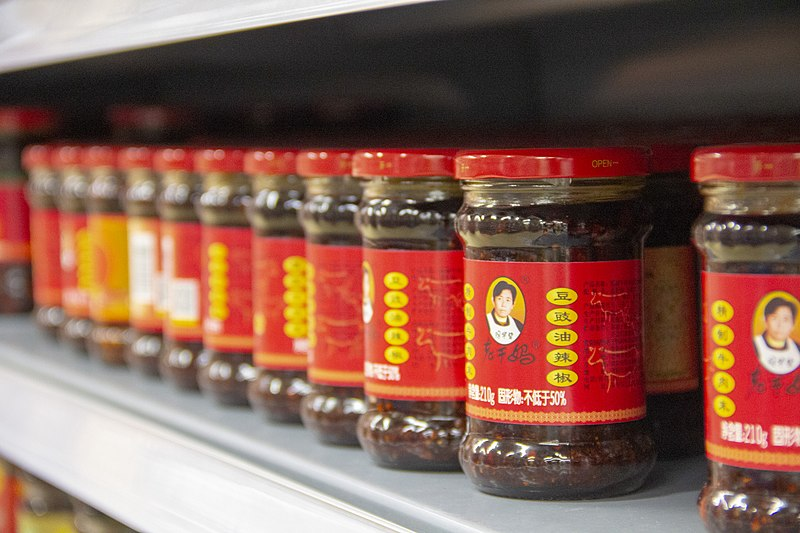
\includegraphics[height=8cm]{./input/module3.jpg}
\end{center}

\vspace{5mm}

\Large *本文的费用估算皆为粗略估算,实际医疗费用应以当地通告为准。

参考文献:

1.宋岩. (n.d.). 抗击新冠肺炎疫情的中国行动. Retrieved July 06, 2020,
from \url{http://www.gov.cn/zhengce/2020-06/07/content_5517737.htm}

2.55万日元!日本治疗1位新冠肺炎患者费用是中国2倍 \&
(5/10)日本疫情状况发布\_检测. (2020, May 10). Retrieved July 06, 2020,
from \url{https://www.sohu.com/a/394276003_658600}

3.在日本住院治疗新冠肺炎需要多少钱?安倍政府将报销费用提高3倍. (2020,
May 26). Retrieved July 06, 2020, from
\url{https://xw.qq.com/cmsid/20200526A0B02E00}

\begin{enumerate}
\def\labelenumi{\arabic{enumi}.}
\setcounter{enumi}{3}
\tightlist
\item
  韩国发布新冠肺炎治疗费用:2万至40万人民币. (n.d.). Retrieved July 06,
  2020, from \url{https://world.huanqiu.com/article/3y9IdVFQWM5}
\end{enumerate}

\vspace{5mm}

\centering
\fontsize{12}{12} \selectfont

\begin{tabular}{ll}


主编:马晶  &  副主编:仁晖,史珂玮 \\
责任编辑: 付铭洲  \\
新闻组:胡睿绮  &  数据分析:宋琰 \\
热点话题:吴舒兰 & 微信排版:韩佩瑾\, 王艺晓 \\
\multicolumn{2}{l}{可视化组:张祺珉\, 刘逸洋\, 周梓淇\, 孙昊\, 唐星鸿\, 齐维为\, 张立达}

\end{tabular}

\end{document}
